%This work is licensed under the Creative Commons Attribution-NonCommercial-NoDerivs 3.0 United States License. To view a copy of this license, visit http://creativecommons.org/licenses/by-nc-nd/3.0/us/ or send a letter to Creative Commons, 444 Castro Street, Suite 900, Mountain View, California, 94041, USA.

\section{Introduction}

In the search for alternative mechanisms to reduce the intrinsic divergence of the electron beam upon photoemission, a possible area of interest was Plasmon-Assisted Photoemission (PAPE). 
This avenue of investigation was motivated by Zawadzka et al \cite{zawadzka_evanescent_2001} who indicate that when driving a surface plasmon on gold they witnessed a reduction in the emission angle of photoemitted electrons.
In their paper, the authors mount a gold foil on a prism; the laser is incident on the gold through the prism.
This geometry is called the Kretschmann geometry.

While this geometry is common, due to fears about the lack of heat conduction through the glass and the power needed to generate a sufficient electron beam current, that UEM applications should explore the ``grating coupling'' geometry.
In this geometry, the plasmon is driven on a periodic surface rather than a flat surface attached to glass.
Futher, in this geometry the back surface is now free to be attached to a heat sink.

\subsection{Driving the Surface Plasmon}

As the name suggests, a plasmon is the quasiparticle of plasma oscillation.
Electrons in a material can couple with electromagnetic fields, in this case a laser field, and oscillate accordingly.
When this occurs at the surface of a material, the resultant quasiparticles are called ``surface plasmon-polaritons.''
Since these will be the only plasmons discussed in this paper, the word ``plasmon'' will be used interchangeably for the name ``surface plasmon-polaritons.''
%TODO should this be formalized, either one way (SPP) or the other

The mathematical formalism of surface plasmon-polaritons is a lengthy subject and well described elsewhere \cite{cottam_introduction_2004,concepts_2002}.

Every material has an intrinsic plasma frequency given by 
\begin{equation}
  \omega_{P} = \sqrt{\frac{\rho_{e} e^2}{\varepsilon_{0} m^*}}
\end{equation}
where $\rho_{e}$ is the electron density and $m*$ is the effective mass of the material.
And in the most simple (undamped) approximations, the dielectric function of the material may be written in terms of this constant.
\begin{equation} \label{eq:dielectric_as_omega}
  \varepsilon(\omega) = 1 - \frac{ \omega_{P}^2 }{ \omega^2 }
\end{equation}

At the interface of a vacuum and such a simple material material, contstraints on the material parameters which may allow surface plasmons result in the condition that the dielectric constant at the oscillation frequency of the surface plasmon $ \varepsilon(\omega_{SP}) = -1 $.
Substituting this result into \ref{eq:dielectric_as_omega} show that this frequency of oscillation is simply related to intrinsic plasma frequency by
\begin{equation}
  \omega_{SP} = \omega_{P} / \sqrt{2}
\end{equation}

Further, plasmons carry momentum whose magnitude is given by
\begin{equation}
  k_{P}^2 = \frac{\omega^2}{c^2} \left( \frac{\varepsilon_{1} \varepsilon_{2}}{\varepsilon_{1} + \varepsilon_{2}} \right)
\end{equation}
but of course for a vacuum interface this is simplified to 
\begin{equation}
  k_{SP}^2 = \frac{\omega^2}{c^2} \left( \frac{ \varepsilon }{ 1 + \varepsilon } \right)
\end{equation}

In order to drive a plasmon on the surface of a material, the portion of the laser wave-vector parallel to the plasmon ($k_{Lx}$) must be matched to the wave-vector of the surface plasmon.
\begin{equation}
  k_{SP} = k_{Lx} + \imath k_{G}
\end{equation}


\section{Experimental Attempts}

\subsection{Commerical Grating on Glass}

For proof-of-concept purposes the first experiment was run on a commercially available gold foil on glass holographic grating.
Like the Kretschmann geometry, a foil on glass grating is vulnerable to heating problems; a plasmon creates a large amount of heat but the glass is a poor heat conductor.
The grating was operational as the angles were tuned attempting to drive the plasmon.
At the instant that the plasmon started, a bright flash was visible on the scintillator screen then disappeared.

After this, the grating showed signs of damage.
\ref{fig:grating-damage} shows the results of Scanning Electron Microscopy (SEM) on the grating.
The damage pattern is round and of the size of the laser spot used to drive the plasmon.
The extent of the damage indicates a large temperature increase, which given the other evidence of the test, can be assumed to be from the sudden appearance of a surface plasmon.

The most important result was that a plasmon was driven successfully; this created the heat that destroyed the grating.
Further this experiment validated the decision not to persue a Kretschmann geometry for fear of heat damage at these high powers.

\begin{figure}
  \centering
  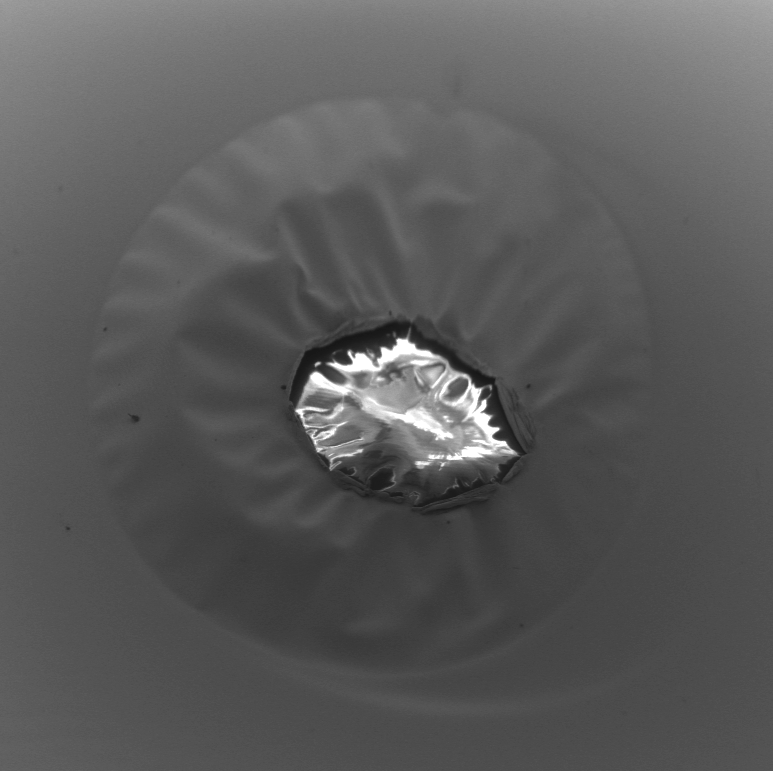
\includegraphics{damage.png}
  \caption{Damage to commerical gold-on-glass holographic grating.}
  \label{fig:grating-damage}
\end{figure}

\subsection{Sinusoidal Grating}

\subsection{Sinusoidal Grating, Rotated}

\subsection{Trenched Grating}
